
\chapter{False Rates for the Baseline and Segmeted Datasets}
\label{appendix:fprfnrother}

\begin{figure}[h]
\centering
\begin{subfigure}[b]{.45\textwidth}
    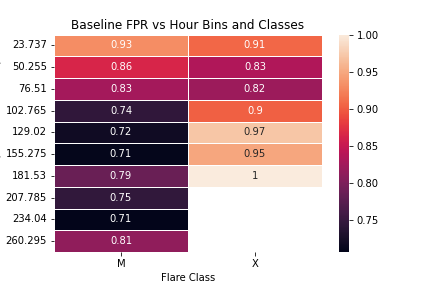
\includegraphics[width=\linewidth]{ThesisFilePkg/figures/findings/baselineFPR.png}
\end{subfigure}
\begin{subfigure}[b]{.45\textwidth}
    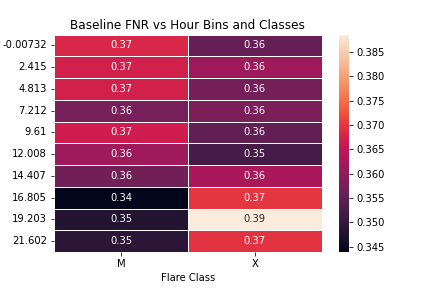
\includegraphics[width=\linewidth]{ThesisFilePkg/figures/findings/baselineFNR.png}
\end{subfigure}
\label{fig:basfr}
\caption{The false negative and positive rates for the baseline dataset. Unlike the segmented dataset, X flares are predicted correctly less frequently than the M class flares.}
\end{figure}


\begin{figure}[h]
\centering
\begin{subfigure}[b]{.45\textwidth}
    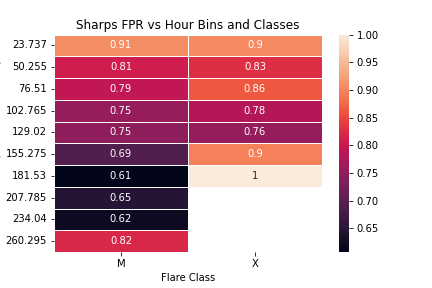
\includegraphics[width=\linewidth]{ThesisFilePkg/figures/findings/sharpsFPR.png}
\end{subfigure}
\begin{subfigure}[b]{.45\textwidth}
    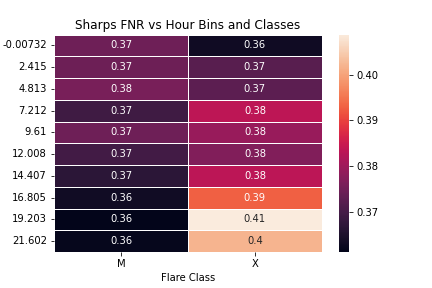
\includegraphics[width=\linewidth]{ThesisFilePkg/figures/findings/sharpsFNR.png}
\end{subfigure}
\label{fig:shpfr}
\caption{The false negative and positive rates for the sharps dataset. Unlike the segmented dataset, X flares are predicted correctly less frequently than the M class flares.}
\end{figure}